\documentclass{standalone}
\usepackage{tikz}

\begin{document}

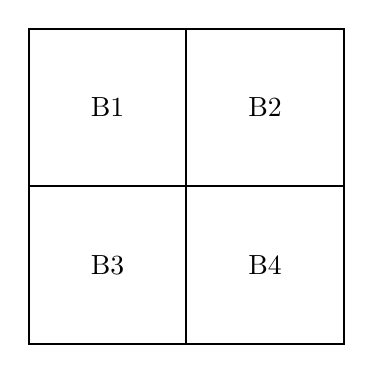
\begin{tikzpicture}

    % Draw the large square
    \draw[thick] (0, 0) rectangle (4, 4);
    
    % Draw the vertical and horizontal lines to divide the square into 4 smaller squares
    \draw[thick] (2, 0) -- (2, 4);
    \draw[thick] (0, 2) -- (4, 2);

    % Add labels inside each small square, numbering from top-left to bottom-right
    \foreach \i in {0,1} {
        \foreach \j in {0,1} {
            % Place label in the center of each block
            \node at (\i*2 + 1, 3 - \j*2) {B\the\numexpr2*\j + \i + 1\relax};
        }
    }

\end{tikzpicture}

\end{document}

